
\subsection*{Frações Parciais}

\begin{frame}
\frametitle{Integração de funções racionais }
\begin{small}

\uncover<1->{Como calcular a integral $\dps\int \frac{2x^3-4x^2-x-3}{x^2-2x-3}dx$ ? }
\bigskip

\uncover<2->{Note que fazendo a divisão dos polinômios obtemos que
$$\int\frac{2x^3-4x^2-x-3}{x^2-2x-3}dx= \int 2x +\frac{5x-3}{x^2-2x-3}dx= x^2+\int \frac{5x-3}{x^2-2x-3}dx.$$
E o problema se reduz a calcular a última integral.}
\bigskip

\uncover<3->{Note que 
$$\frac{5x-3}{x^2-2x-3}=\frac{2}{x+1}+\frac{3}{x-3}.$$
Portanto podemos calcular a integral!}

\end{small}
\end{frame}

\begin{frame}[fragile=singleslide]{}
	Obviamente o python é capaz de calcular essa integral diretamente
\begin{block}{ }
	\begin{pyverbatim}
from sympy import *

x=symbols('x')

integrate((2*x**3-4*x**2-x-3)/(x**2-2*x-3),x)
\end{pyverbatim}
\end{block}
\begin{pycode}
from sympy import *

x=symbols('x')

int=integrate((2*x**3-4*x**2-x-3)/(x**2-2*x-3),x)
\end{pycode}
\[\int \frac{2x^3-4x^2-x-3}{x^2-2x-3}dx=\py{sp.latex(int)}+C\]
\end{frame}

\begin{frame}[fragile=singleslide]{}
Entretanto, o comando apart do sympy, nos permite decompor o integrando para que possamos resolvê-lo com a técnica apresentada:
\begin{block}{ }
\begin{pyverbatim}
from sympy import *

apart((2*x**3-4*x**2-x-3)/(x**2-2*x-3),x)
\end{pyverbatim}
\end{block}
\begin{pycode}
from sympy import *
frac=apart((2*x**3-4*x**2-x-3)/(x**2-2*x-3),x)
\end{pycode}
\[\frac{2x^3-4x^2-x-3}{x^2-2x-3}dx=\py{latex(frac)}\]
\end{frame}



%\begin{frame}{Crescimento Populacional Logístico}
%Vimos que um modelo simples de crescimento populacional é aquele em que se supõe que a taxa de crescimento de uma população \textcolor{blue}{$\frac{dy}{dt}$} é proporcional à população presente \textcolor{blue}{$y(t)$} naquele instante.	O \dt{crescimento logístico}, leva em conta que a população tem um valor máximo sustentável \textcolor{red}{$M$}. Quando a população se aproxima da capacidade máxima, os recursos tornam-se menos abundantes e a taxa de crescimento começa a diminuir. Uma relação simples  que exibe esse comportamento é quando 
%	\[\textcolor{blue}{\frac{dy}{dt}}={\color{orange}k}\textcolor{blue}{y}(\textcolor{red}{M}-\textcolor{blue}{y}) \]
%	
%%\begin{exe} Biólogos colocaram em um lago 400 peixes e estimaram a capacidade de suporte como 10.000. O número de peixes triplicou no primeiro ano. Encontre uma expressão para o tamanho da população de peixes depois de $t$ anos.
%%\end{exe}	
%Usando-se o método de frações parciais, pode-se mostrar que a população é modelada por:
%\[{\color{blue}y(t)}=\frac{{\color{red}M}}{1+Ce^{-{\color{orange}k}{\color{red}M}t}},\ t\geq 0.\]
%
%
%\end{frame}
%
%\begin{frame}
%\begin{exe}
%Em uma comunidade de 45.000 pessoas, a taxa de crescimento de uma epidemia de gripe é conjuntamente proporcional ao número de pessoas que a contraíram e ao número de pessoas que não a contraíram. 
%
%\begin{enumerate}
%\item Se 200 pessoas tiveram a gripe quando irrompeu a epidemia e 3.000 tiveram gripe 3 semanas depois, ache um modelo que descreva a epidemia.
%
%\item Qual o número estimado de pessoas terá a gripe após 5 semanas?
%
%\item Em quanto tempo a gripe atingirá metade da população?
%\end{enumerate}
%
%\end{exe}
%\end{frame}
%
%\begin{frame}
%No exemplo anterior, se $y(t)$ é o número de centenas de pessoas infectadas no instante $t$, então
%\[y(t)=\frac{450}{1+224(16)^{-t/3}},\ t\geq 0.\]
%
%
\includegraphics[scale=0.6]{figuras/fig-gripe.png}
%
%\end{frame}



%\begin{frame}
%\frametitle{Método das Frações Parciais }
%\begin{small}
%
%\uncover<1->{Vejamos através de alguns exemplos como aplicar o Método ds fracões parciais para calcular integrais racionais. 
%\begin{enumerate}
%\item $\dps\int \frac{x^2+4x+1}{(x-1)(x+1)(x+3)}dx$
%\item $\dps\int \frac{x-1}{(x+1)^3}dx$
%\item $\dps\int \frac{-2x+4}{(x^2+1)(x-1)^2}dx$
%\item $\dps\int \frac{dx}{x(x^2+1)^2}dx$
%\end{enumerate}}
%
%\end{small}
%\end{frame}


%\begin{frame}{Controlando uma população}
%\begin{minipage}{0.6\textwidth}
%O \dt{javaporco}\footnotemark, resultado do cruzamento entre o javali e o porco, é considerado uma praga para a agricultura. Por esta razão, o javali (incluindo o javaporco) é a única espécie cuja caça é permitida por lei no Brasil. 
%\end{minipage}
%\begin{minipage}{0.3\textwidth}
%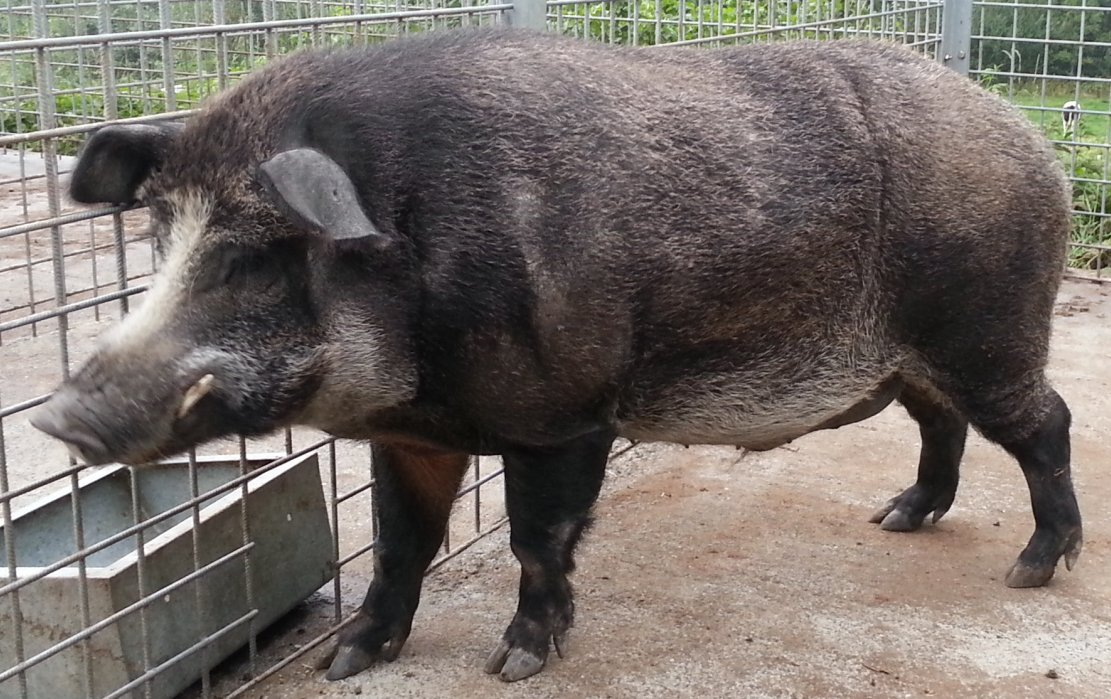
\includegraphics[scale=0.1]{javaporco.jpg}
%\end{minipage}
%
%\begin{block}{Modelo Matemático}
%Se considerarmos que uma população é extinta quando cai abaixo de um certo nível \textcolor{orange}{$m$} e que tem um valor máximo sustentável \textcolor{red}{M}, isto é, a taxa de crescimento diminui com a falta de recursos, um modelo matemático que descreve o crescimento dessa população é:
%\[\frac{dy}{dt}=ky(\textcolor{red}{M}-y)(y-\textcolor{orange}{m)}.\]
%\end{block}
%
%\footnotetext[1]{Em 2018 o javaporco foi \href{https://piaui.folha.uol.com.br/um-javaporco-no-caminho-do-governador-de-sao-paulo/}{notícia na revista piauí} por atrapalhar a campanha do candidado a governador Márcio França em SP.}
%\end{frame}
%

\begin{frame}{ }

\begin{casa}
Calcule \begin{enumerate}
\item $\dps\int\frac{2x^3-2x^2+1}{x^2-x}dx$
\item $\dps\int \frac{x^2+4x+1}{(x-1)(x+1)(x+3)}dx$
\end{enumerate}


%\begin{enumerate}
%\item $\dps \int \frac{x^2-4x-4}{x^3-2x^2+4x-8}dx$
%\item 
%\end{enumerate}

\end{casa}

\end{frame}

%\begin{frame}
%
%\begin{exer}
%Um dia em um campus universitário com 5\,000 alunos, onde se esperava uma assembleia estudantil um aluno ouviu que certo estudante polêmico iria fazer, durante a assembleia, um discurso explosivo. Essa informação foi transmitida para amigos que, por sua vez, a transmitiram a outros. A taxa com que se espalhou essa informação é conjuntamente proporcional ao número de pessoas que a ouviram e ao número de pessoas que não a ouviram. Se após 10 min 144 pessoas ouviram a informação, ache o modelo matemático que escreve a divulgação da notícia. Em quanto tempo metade das pessoas terão ouvido a notícia? 
%\end{exer}
%
%\end{frame}





